%% What VeReMi Measures --- structural artefacts in VANET misbehaviour benchmarks
%%
%% Target venue: ISOC VehicleSec (Symposium on Vehicle Security and Privacy).
%% VehicleSec uses the NDSS class. Swap the first line for \documentclass{ndss} when the
%% class file is available. IEEEtran is used here because it is portable and compiles anywhere.
\documentclass[conference]{IEEEtran}

\usepackage{booktabs}
\usepackage{array}
\usepackage{graphicx}
\usepackage{url}
\usepackage{amsmath}
\usepackage[hidelinks]{hyperref}

\begin{document}

\title{What VeReMi Measures: Structural Artefacts in\\ VANET Misbehaviour Detection Benchmarks}

\author{\IEEEauthorblockN{Hannan Muzammil}
\IEEEauthorblockA{Hannsoft\\ \url{https://www.hannsoft.org/}\\ abdullhannan0311@gmail.com}}

\maketitle

\begin{abstract}
One untrained scalar solves six of eight VeReMi archives.
It reads message timing alone, never a claimed position.
These archives are the field's main shared misbehaviour benchmark.
Reported detection rates on them sit between 94\% and 99.9\%.
We audit them by measurement: every claim is re-derived from source.
We examine the eight Sybil archives of the extension.
Pseudonyms encode the true sender in 86.5--100\% of identity pairs.
No benign vehicle in them emits a second pseudonym.
Attacker prevalence is 30.0\% of vehicles in all eight.
Attacker identities form 68--98\% of the identity population.
Ground-truth files list up to 28 times fewer identities than receivers observe.
We then run one detector through seven progressively stricter protocols.
Removing ground-truth aggregation is associated with a 0.060 fall.
We evaluate the pseudonym feature in its original representation.
The lowest stable evaluable prevalence is 3\% dense, 5\% sparse.
Ranking metrics barely move with prevalence; precision metrics collapse.
We show VeReMi 2018 cannot validate signal-strength position verification.
Its measured path-loss exponent is 0.93 against a free-space two.
That detector then reaches AUC 0.530, barely above chance.
We release code, controls and a reporting checklist for future work.
\end{abstract}

\begin{IEEEkeywords}
VANET, misbehaviour detection, Sybil attack, benchmarking, reproducibility, VeReMi.
\end{IEEEkeywords}

\begin{figure}[t]
\centering
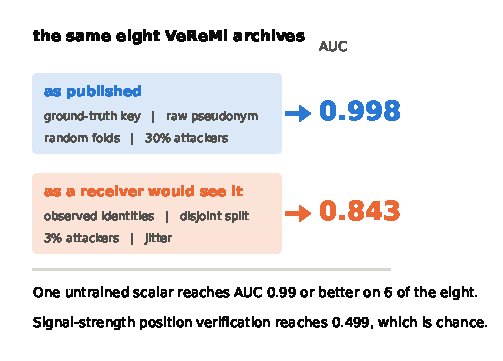
\includegraphics[width=\columnwidth]{fig_abstract.pdf}
\caption{The same archives under two protocols.
The upper lane is practice reconstructed from the corpus.
The lower lane removes each advantage a receiver could not have.
Values are GridSybil dense, the family that resists the shortcuts.
Both are read from the result files, not quoted.}
\label{fig:abstract}
\end{figure}

\section{Introduction}

A Sybil attacker presents many identities from one radio.
In vehicular networks the consequence is direct and physical.
Safety applications count reporters before believing a claim.
Fake congestion, forged warnings and vote manipulation all follow.
Douceur formalised the problem for peer-to-peer systems~\cite{douceur2002}.
Newsome adapted the defence taxonomy to sensor networks~\cite{newsome2004}.
Vehicular work inherited both, then grew for twenty years.

Progress is normally judged by reported detection rates.
Those rates have risen steadily and now approach saturation.
Early trajectory schemes reported roughly 98\% detection~\cite{chang2011}.
Recent deep models report between 94\% and 99.9\%.
Such numbers imply the problem is essentially solved.
Deployment experience does not support that conclusion.

Security machine learning has met this pattern before.
Sommer and Paxson warned about it fifteen years ago~\cite{sommer2010}.
Arp et al.\ catalogued the pitfalls that produce it~\cite{arp2022}.
Sampling bias and spurious correlation head their list.
We found that lens rarely applied to vehicular benchmarks.

Comparability is the missing ingredient, and it is scarce.
VeReMi introduced a common reference for misbehaviour detection~\cite{heijden2018}.
Its extension added attack families including explicit Sybil variants~\cite{kamel2020}.
Shared evaluation is nonetheless rare in this literature.
Of our 92 full texts, 5 mention VeReMi at all.
Only 7 name any public dataset whatsoever.
The remaining 92\% name no public dataset at all.
So these archives are not ubiquitous; they are the main alternative.
That is precisely why their contents matter.

Figure~\ref{fig:abstract} summarises what follows.
We therefore ask what these archives actually contain.
We parse them and quantify their structure directly.
We then re-derive headline results under explicit controls.
Our contributions are as follows.

\begin{itemize}
  \item We document six structural artefacts across all eight Sybil archives.
        Each is measured from source, not read from documentation.
  \item We show a single untrained scalar solves most archives.
        No training, no linkage and no physical reasoning are required.
  \item We separate timing evidence from geometric evidence.
        Timing alone reaches AUC near unity on several families.
  \item We run one detector through seven progressively stricter protocols.
        Each stage measures the change associated with one removed control.
  \item We sweep prevalence, jitter, attack intensity and beacon rate.
  \item We show VeReMi 2018 cannot validate signal-strength verification.
  \item We release controls, scripts and a reporting checklist.
\end{itemize}

Our stance is deliberately narrow.
We do not accuse any author of exploiting a loophole.
The published protocols we reconstruct were reasonable when written.
The defensible claim is simpler and more uncomfortable.
These benchmarks substantially simplify the intended deployment task.

\section{Background and Related Work}

\subsection{Sybil detection in vehicular networks}

Early vehicular defences used physics rather than cryptography.
Xiao et al.\ verified claimed positions from signal-strength distributions~\cite{xiao2006}.
Guette and Ducourthial then quantified the attacker's freedom~\cite{guette2007}.
Transmit power tuning and directional antennas defeat naive checks.
Bouassida et al.\ measured signal variation against real hardware~\cite{bouassida2009}.

Infrastructure-anchored designs followed.
Park et al.\ used roadside timestamp series instead of certificates~\cite{park2009}.
Footprint made anonymous roadside proofs into a trajectory identity~\cite{chang2011}.
P2DAP detected pseudonym reuse while preserving anonymity~\cite{zhou2007,zhou2011}.
Later work extended these ideas to conspiring attackers~\cite{feng2016}.

Statistical and learning approaches then dominated.
Voiceprint compared signal-strength series without a propagation model~\cite{yao2017}.
Ayaida et al.\ detected contradictions against a traffic-flow model~\cite{ayaida2019}.
Dutta and Chellappan clustered platoon dispersion over time~\cite{dutta2013}.
Grover et al.\ combined several verification variables~\cite{grover2015}.
Yu et al.\ consolidated the position-verification line~\cite{yu2013}.
Recent systems use ensembles, graphs and gradient boosting~\cite{azam2022,sefati2025}.

A parallel line prices identities instead of detecting them.
Baza et al.\ required proofs of work and location~\cite{baza2020}.
Khatri et al.\ anchored location proofs on a blockchain~\cite{khatri2024}.
Hadri et al.\ used verifiable delay functions with fog nodes~\cite{hadri2026}.
Credential designs prevent concurrency outright~\cite{funderburg2021,akil2023}.
Fog and 5G variants target lightweight deployment~\cite{almazroi2024}.

Surveys cover this ground thoroughly.
Boualouache and Engel survey machine-learning misbehaviour detection~\cite{boualouache2023}.
A recent survey covers federated and edge approaches~\cite{tits2025survey}.
We therefore do not attempt another survey.

\subsection{What our critique would touch}

Table~\ref{tab:touch} lists representative recent work.
Two of the five evaluate on VeReMi.
The other three use their own simulations.
For each we name the protocol choice our results bear on.
We are not re-running their systems or disputing their code.
We ask only whether their evaluation would survive our controls.

\begin{table}[t]
\caption{Representative recent work and the control it lacks.
Only the first and third rows evaluate on VeReMi.}
\label{tab:touch}
\centering
\footnotesize
\begin{tabular}{@{}>{\raggedright\arraybackslash}p{1.75cm}>{\raggedright\arraybackslash}p{2.6cm}>{\raggedright\arraybackslash}p{2.55cm}@{}}
\toprule
Work & Protocol as described & Control absent \\
\midrule
Azam \cite{azam2022}      & per-node features, random folds & vehicle-disjoint split \\
Sefati \cite{sefati2025}  & spatio-temporal model & single-scalar baseline \\
Tay\c{s}i \cite{taysi2025}& signal-strength similarity      & calibrated power \\
Almesaeed \cite{almesaeed2025} & channel characterisation   & calibrated power \\
Morton \cite{morton2024}  & trust aggregation               & prevalence sweep \\
\bottomrule
\end{tabular}
\end{table}

Azam et al.\ aggregate movement features per node, then apply random folds.
That is exactly the first protocol in our cascade.
Guven and Tay\c{s}i built a new dataset for related reasons~\cite{guven2024}.
Their motivation and ours agree on the substrate problem.

\subsection{Benchmarks and their scrutiny}

VeReMi was created to make results comparable~\cite{heijden2018}.
Its extension added Sybil families and more scenarios~\cite{kamel2020}.
Evaluation practice around them is rarely examined.

A newer release has since appeared~\cite{nextgen2026}.
VeReMi NextGen moves to the InTAS scenario and adds attacks.
It ships predefined training and validation splits.
Its aliases do not encode the sender: at most 0.02\%.
That single change removes our first structural artefact.
Our structural audit concerns VeReMi and its extension.
Section~\ref{sec:generalise} carries the same measurements to NextGen.
A full audit of NextGen is future work, not this paper.

Table~\ref{tab:datasets} places the four artefacts side by side.
It also states what this audit adds to each.

\begin{table}[t]
\caption{The four public artefacts, and what we add.
Sybil means explicit Sybil families, not misbehaviour generally.}
\label{tab:datasets}
\centering
\scriptsize
\begin{tabular}{@{}>{\raggedright\arraybackslash}p{1.7cm}ccc>{\raggedright\arraybackslash}p{2.0cm}@{}}
\toprule
Artefact & Sybil & RSSI & Rotation & What we add \\
\midrule
VeReMi \cite{heijden2018} & no & yes & no & path loss and detector \\
Extension \cite{kamel2020} & yes & no & no & artefacts, cascade, sweeps \\
Guven \cite{guven2024} & yes & yes & --- & availability status only \\
NextGen \cite{nextgen2026} & yes & no & no & first structural probe \\
\bottomrule
\end{tabular}
\end{table}

Only the Guven set pairs Sybil attacks with received power.
We could not evaluate it, for the reason given later.
We found no study in our search that measures them structurally.

Adjacent work does question evaluation.
SixPack evades detectors by abusing anti-lock braking signals~\cite{sixpack2021}.
That work targets detectors, not the dataset itself.
Iwendi et al.\ illustrate the reported-accuracy pattern we examine~\cite{iwendi2018}.
We found no study in our search that measures these archives structurally.

\subsection{Why realism matters}

Attack impact depends strongly on attacker share.
S\"oderh\"all et al.\ measured navigation-service manipulation~\cite{soderhall2025}.
Sybils at 3\% of users raised average travel time 20\%.
Our search found no field measurement of deployed V2X prevalence.
Neither 3\% nor 30\% is an observed field figure.
The honest response is a sweep, which we report.
Physical-layer methods stay popular despite substrate limits~\cite{taysi2025,almesaeed2025}.

\section{Method}

\subsection{Corpus}

We assembled 331 records on vehicular Sybil attacks.
Sources were OpenAlex, Semantic Scholar, arXiv, OpenAIRE and HAL.
The index was built on 3 September 2026.
Records span publication years 2006 to 2026.

Screening kept work on Sybil attacks in vehicular networks.
We deduplicated on digital object identifier and on title.
Records without a reachable open-access file were kept for counting only.
Ninety-two open-access full texts were obtained and parsed.
We extracted reported experimental parameters by pattern matching.

The flow is therefore 331 records screened, 92 full texts analysed.
We report it in that form rather than as a systematic review.
Two requirements of such a review are not met here.
The exact query strings were not preserved during collection.
Screening was done by one author without a second rater.
We state both gaps rather than describe the search as systematic.

The corpus supplies context, not the paper's main claims.
It is a convenience sample, not an exhaustive review.
Statements below about absent prior work refer to this search.

\subsection{Datasets and their schema}

Three public artefacts form the substrate, verified by MD5 against Zenodo.
A fourth, VeReMi NextGen, is used only in Section~\ref{sec:generalise}.
VeReMi 2018 provides received power and position falsification attacks.
Its record is \url{10.5281/zenodo.20081895}.
VeReMi Extension provides Sybil families and pseudonyms.
Its record is \url{10.5281/zenodo.20090854}.
A preprocessed derivative provides ready-to-use feature rows.
Its record is \url{10.5281/zenodo.14903687}.
All three are CC-BY licensed.
We name the records because titles alone are ambiguous.

Table~\ref{tab:schema} lists every field we read.
The third column is our central methodological device.
A field is public if a receiver could observe it.
Everything else is evaluation-only and never reaches a model.

\begin{table}[t]
\caption{Fields read, and who may see them.}
\label{tab:schema}
\centering
\footnotesize
\begin{tabular}{llc}
\toprule
Field & Meaning & Detector sees \\
\midrule
\texttt{type} & record kind, 2/3/4 & yes \\
\texttt{rcvTime} & reception time & yes \\
\texttt{sendTime} & claimed send time & yes \\
\texttt{messageID} & transmission identifier & yes \\
\texttt{pos}, \texttt{pos\_noise} & claimed position, variance & yes \\
\texttt{spd}, \texttt{spd\_noise} & claimed speed, variance & yes \\
\texttt{acl}, \texttt{acl\_noise} & claimed acceleration & yes \\
\texttt{hed}, \texttt{hed\_noise} & claimed heading & yes \\
\texttt{RSSI} & received power, 2018 only & yes \\
receiver id & from the log filename & metadata \\
\midrule
\texttt{senderPseudo} & raw pseudonym & \textbf{hashed first} \\
\texttt{sender} & true vehicle identifier & \textbf{no} \\
\texttt{A}$n$ in filename & attack type label & \textbf{no} \\
\bottomrule
\end{tabular}
\end{table}

\subsection{Preprocessing}

The pipeline has five steps and no hidden state.

\begin{enumerate}
  \item Parse every receiver log in every simulation window.
  \item Replace each pseudonym with \texttt{BLAKE2b(salt, archive, pseudonym)}.
  \item Deduplicate on \texttt{messageID} within a window.
  \item Build features per identity, or per identity pair.
  \item Split by true vehicle, then fit and score.
\end{enumerate}

Step three matters more than it looks.
Each transmission is logged once per receiver that heard it.
Median duplication is six copies in the dense archives.
Grouping across receivers destroys cadence and inflates timing features.

Step five uses the true vehicle for splitting and scoring only.
Both endpoints of a pair must fall on one side.
Grouping on one endpoint lets the other straddle the split.
We assert disjointness at run time rather than trusting the splitter.

\subsection{Detector and features}

Everything here runs on one desktop machine.
The cascade takes about two hours across eight archives.
Every other experiment finishes in minutes.

One classifier is used throughout, deliberately.
It is a random forest of 200 trees, minimum leaf two.
Scikit-learn supplies it, with the seed fixed per run.
We do not tune it, because tuning is not the question.
A stronger model could shift the absolute values.
Whether it would shift the differences we report is untested.

Table~\ref{tab:features} lists the four feature sets.
The timing and geometry split carries our central ablation.
Readers can therefore contest the partition rather than trust it.

\begin{table}[t]
\caption{Feature sets. Pair features describe two identities;
identity features describe one.}
\label{tab:features}
\centering
\footnotesize
\begin{tabular}{@{}>{\raggedright\arraybackslash}p{1.35cm}>{\raggedright\arraybackslash}p{6.1cm}@{}}
\toprule
Set & Members \\
\midrule
Pair, geometry & mean, minimum and standard deviation of inter-claim distance;
mean absolute speed difference; speed correlation \\
Pair, timing & presence overlap; comparison count; median nearest-claim gap;
phase residual against the beacon period \\
Identity, rate & message count; duration; median and deviation of inter-arrival \\
Identity, kinematic & speed mean, deviation and maximum; acceleration mean and
deviation; position span in each axis; step mean and deviation; kinematic
residual; reported position and heading noise \\
\bottomrule
\end{tabular}
\end{table}

Pair candidates are identities co-observed by one receiver.
We compare only claims within one second of each other.
A pair is positive when both identities share a true vehicle.
The linkage experiment scores 1\,588 to 29\,218 pairs per archive.
Positive rates run from 2.7\% to 10.5\%.

\subsection{Metrics}

We report ROC-AUC and average precision.
Both are implemented twice and cross-checked at every call.
The first implementation is the normalised Mann--Whitney statistic.
The second is scikit-learn, and a run aborts on disagreement.
Ties receive mid-ranks, where naive implementations usually diverge.
On tied and adversarial inputs the two agree to machine precision.

Three interval kinds appear, and they are not interchangeable.
A percentile bootstrap over test rows measures sampling error.
DeLong intervals check that bootstrap on the physical-layer result.
Spread across random seeds is reported as a subscript instead.
Each estimate is printed only beside an interval for itself.

\section{Corpus Reporting Practice}

Table~\ref{tab:reporting} summarises what the 92 papers report.
The pattern is not primarily statistical weakness.
Most papers omit the parameters needed for interpretation.

\begin{table}[t]
\caption{Reported items across the 92 full texts.
Counts are regular-expression matches over the whole text.
A match is an upper bound: the item appears somewhere, not necessarily usably.}
\label{tab:reporting}
\centering
\footnotesize
\begin{tabular}{@{}lr@{}}
\toprule
Reported item & Papers \\
\midrule
Explicit threat model & 22 \\
Vehicle count & 34 \\
Simulation time & 18 \\
Beacon rate & 9 \\
Attacker fraction & 9 \\
Simulation area & 6 \\
ROC or AUC & 4 \\
Any significance test or interval & 2 \\
Repository or archive link & 3 \\
Adversarial machine learning content & 0 \\
\bottomrule
\end{tabular}
\end{table}

Only nine papers state their beacon rate.
Only nine state the attacker fraction used.
Both quantities change task difficulty substantially.
Four mention a ROC curve or an area under one.
Two report any interval or significance test.

Three papers give a repository or archive link.
All three point at the same archive.
That archive was restricted when we sought access.
No paper in the corpus offered code we could run.
Eleven papers published since 2021 mention ns-2.
One of the eleven is a survey citing it in passing.
That simulator stopped active development in 2011.

\section{Structural Artefacts}

Table~\ref{tab:census} is the complete census.
Every column is measured from the raw archives.
The scripts producing it import none of our loader.

\begin{table*}[t]
\caption{Complete census of the eight VeReMi Extension Sybil archives, measured from source.}
\label{tab:census}
\centering
\footnotesize
\begin{tabular}{lrrrrrrrr}
\toprule
Archive & Vehicles & Attacker & Prevalence & Identities & Attacker & Identity & Encoding & Copies per \\
        &          & vehicles & (vehicles) &            & identities & prevalence & rate & transmission \\
\midrule
GridSybil dense            & 4\,064 & 1\,219 & 30.00\% & 8\,793   & 5\,948   & 67.6\% & 86.5\% & 6 \\
GridSybil sparse           & 1\,688 & 507    & 30.04\% & 3\,726   & 2\,545   & 68.3\% & 87.0\% & 4 \\
DataReplaySybil dense      & 4\,067 & 1\,221 & 30.02\% & 72\,140  & 69\,294  & 96.1\% & 100\%  & 7 \\
DataReplaySybil sparse     & 1\,688 & 507    & 30.04\% & 27\,421  & 26\,240  & 95.7\% & 100\%  & 4 \\
DoSRandomSybil dense       & 4\,067 & 1\,221 & 30.02\% & 112\,191 & 109\,345 & 97.5\% & 100\%  & 7 \\
DoSRandomSybil sparse      & 1\,688 & 507    & 30.04\% & 47\,473  & 46\,292  & 97.5\% & 100\%  & 4 \\
DoSDisruptiveSybil dense   & 4\,067 & 1\,221 & 30.02\% & 112\,187 & 109\,341 & 97.5\% & 100\%  & 7 \\
DoSDisruptiveSybil sparse  & 1\,688 & 507    & 30.04\% & 47\,466  & 46\,285  & 97.5\% & 100\%  & 4 \\
\bottomrule
\end{tabular}

\vspace{2pt}
\footnotesize Identities per attacker, median and maximum: GridSybil 3/7 dense and 6/7 sparse;
DataReplaySybil 56/100 dense and 50/100 sparse; both denial-of-service families 100/100.
\end{table*}

\subsection{Pseudonyms encode sender identity}

Received messages carry both a true sender and a pseudonym.
A receiver observes only the pseudonym in deployment.
We compared the two fields across every record.

Six archives encode the sender in every identity pair.
Both GridSybil archives encode it in 86.5\% and 87.0\%.
Sender 15 emits pseudonyms 10155 and 20155.
Sender 5853 emits 1058535 and 2058535.
The construction resembles $k\cdot10^{n}+\text{sender}\cdot10+c$.

Two consequences follow.
Grouping identities becomes solvable by string arithmetic alone.
More subtly, many pipelines aggregate features per true sender.
That hands the model the partition it should infer.

The GridSybil shortfall has a single cause.
One pseudonym is shared by many distinct senders.
Its value is the literal integer one.
It carries 147\,672 ground-truth messages in the dense archive.
Any pipeline keyed on the pseudonym merges those vehicles silently.

\subsection{The pseudonym decodes to its owner}

The previous subsection is a claim about string structure.
We turn it into a decoder and measure what it recovers.

The decoder is deliberately trivial and untrained.
It returns the longest sender identifier found inside the pseudonym.

The control keeps both populations and breaks the correspondence.
For decoding, vehicles are permuted among pseudonyms.
For linkage, pseudonyms are permuted among identities.
A leak shows as a gap between the real and permuted arms.

\begin{table}[t]
\caption{Recovering the sender from the pseudonym alone.
Decode accuracy names the exact emitting vehicle.
Linkage asks whether two pseudonyms share one vehicle.}
\label{tab:decode}
\centering
\footnotesize
\begin{tabular}{@{}lrrr@{}}
\toprule
Measure & Real & Permuted & Chance \\
\midrule
Decode accuracy, mean & 0.876 & 0.0031 & 0.0011 \\
Decode accuracy, range & 0.771--1.000 & --- & --- \\
Linkage AUC, range & 0.999--1.000 & 0.444--0.608 & 0.5 \\
\bottomrule
\end{tabular}
\end{table}

\begin{figure}[t]
\centering
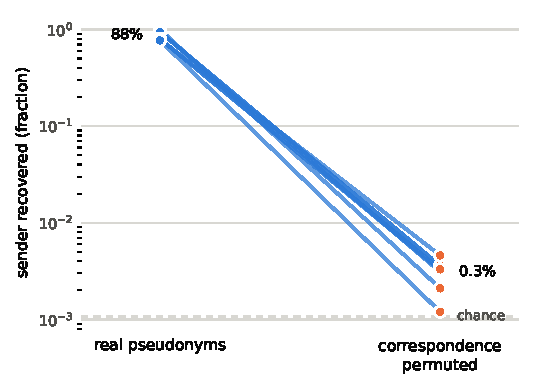
\includegraphics[width=\columnwidth]{fig_decode.pdf}
\caption{Recovering the sender from the pseudonym alone.
Each line is one archive, on a logarithmic axis.
The left point uses real pseudonyms, the right permuted ones.
Permuting keeps both populations and breaks only the correspondence.
The dashed rule marks chance for these populations.}
\label{fig:decode}
\end{figure}

%%DECODE_TEXT%%

%%INFORMATION%%

\subsection{Benign vehicles do not change pseudonyms}

We counted identities per vehicle in the eight Sybil archives.
Labels came from filenames over the complete member list.
Not one benign vehicle emits a second pseudonym.
The benign maximum is exactly one across all eight.

F2MD generated these archives and supports pseudonym change policies.
Our claim is about the eight Sybil archives we examined.
We make no claim about other Extension scenarios or configurations.
The policies exist in the generator; they are not exercised here.

One alternative reading would invalidate the measurement.
Rotation might occur while the logged sender identifier also changes.
The mapping would then be one to one by construction.
Renewing the identifier would truncate every observed lifetime.
Lifetimes would cluster near the policy period.

They do not.
Benign observation spans have median 90.5 to 94.0 seconds.
Their coefficient of variation is 0.52 to 0.57.
No single value holds more than 1.8\% of vehicles.
The spread follows radio dwell time, not a fixed schedule.
We therefore read the mapping as genuine, not as renaming.

Pseudonym change is absent for honest vehicles in these archives.
Unlinkability and pseudonym lifetime cannot be studied on them.
Attackers, by contrast, hold many identities each.
Identity count alone then separates the classes almost perfectly.

\subsection{Ground truth omits most attacker pseudonyms}

This artefact is easy to inherit without noticing.
The ground-truth files list one pseudonym per vehicle.
That holds for attacker vehicles too, in seven archives.
The receiver logs tell a very different story.

For DoSRandomSybil dense the two disagree by 27.6 times.
Ground truth names 4\,068 identities; the logs show 112\,191.
The discrepancy is in the identity representation only.
Both views contain the same 1\,221 attacker vehicles.
What ground truth omits is the pseudonyms those attackers emitted.
Deriving the Sybil partition from ground truth alone therefore finds nothing.
We build labels from receiver logs and filenames instead.

\subsection{Attacker prevalence is fixed and unrealistic}

Attacker share is 30.0\% of vehicles in every archive.
The eight values span 30.00\% to 30.04\%.
Identity-level prevalence is different and much higher.
It ranges from 67.6\% to 97.5\% across the archives.

Our search found no field measurement of V2X prevalence.
Thirty percent is not defended anywhere in the documentation.
Impact is already severe at 3\% in navigation services~\cite{soderhall2025}.
We therefore treat prevalence as a variable, not a constant.

\subsection{Attack intensity varies by two orders}

Identities per attacker differ sharply between families.
GridSybil attackers hold one to seven identities.
The other families reach one hundred identities.
Papers rarely name the family they evaluated.

\subsection{The preprocessed derivative cannot express the task}

One popular derivative offers 2.27 million ready rows.
It contains no sender and no pseudonym column.
Sybil detection is therefore impossible on it in principle.
Nineteen attack types and one benign class are balanced exactly.
Row-level attacker prevalence is therefore 95\%.

Its receiver column is separately malformed.
Just two identifiers account for 95.0\% of the rows.
The other 113\,477 identifiers hold exactly one row each.
Receiver-disjoint validation then degenerates without warning.
One split in five gave accuracy 1.000 with F1 0.000.
Its test fold contained a single class.

\section{How Far the Task Is Simplified}

\subsection{One scalar solves most archives}

We computed two statistics per identity.
The first is median inter-arrival time.
The second is raw message count.
Neither requires training, linkage or physical reasoning.

Direction is fixed before looking at any score.
An attacker splits one budget across many ghosts.
Each ghost therefore transmits less often, not more.
We score larger interval and smaller count as attacker.
Table~\ref{tab:scalar} gives both statistics per archive.

\begin{table}[t]
\caption{Single-scalar separation, all eight archives.
Benign identities beacon at 1.0\,s throughout.
Brackets give the bootstrap 95\% interval.}
\label{tab:scalar}
\centering
\footnotesize
\begin{tabular}{lll}
\toprule
Archive & AUC interval & AUC count \\
\midrule
GridSybil dense           & 0.657\,[.631,.682] & 0.635\,[.608,.662] \\
GridSybil sparse          & 0.576\,[.550,.604] & 0.601\,[.572,.629] \\
DataReplaySybil dense     & 0.544\,[.531,.557] & \textbf{0.996}\,[.992,.999] \\
DataReplaySybil sparse    & 0.534\,[.520,.549] & \textbf{0.993}\,[.989,.997] \\
DoSRandomSybil dense      & \textbf{1.000}\,[1.00,1.00] & 0.996\,[.992,.999] \\
DoSRandomSybil sparse     & \textbf{1.000}\,[1.00,1.00] & 0.994\,[.989,.997] \\
DoSDisruptiveSybil dense  & \textbf{1.000}\,[.999,1.00] & 0.996\,[.992,.999] \\
DoSDisruptiveSybil sparse & \textbf{1.000}\,[.999,1.00] & 0.994\,[.989,.997] \\
\bottomrule
\end{tabular}
\end{table}

%%BUDGET%%
Only the two GridSybil archives resist both trivial statistics.

\subsection{Timing evidence versus geometric evidence}

We next linked identity pairs to one vehicle.
Splits were vehicle-disjoint and transmissions were deduplicated.
Features were partitioned into timing and geometry.

\begin{figure}[t]
\centering
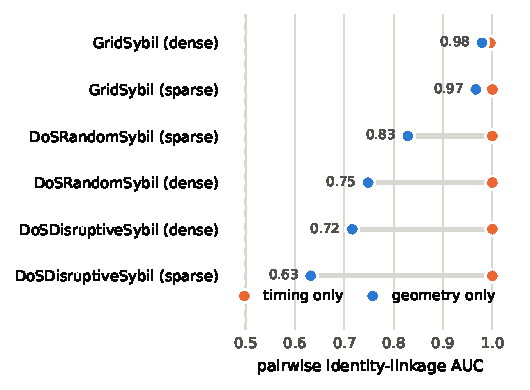
\includegraphics[width=\columnwidth]{fig_ablation.pdf}
\caption{Timing evidence versus geometric evidence, per archive.
Each pair shows one archive under two feature sets.
Timing alone sits at or near AUC 1.000 everywhere.
Geometry, the physically meaningful signal, varies widely.
The dashed rule marks chance at AUC 0.5.
DataReplaySybil is absent: it yields no concurrent pairs.}
\label{fig:ablation}
\end{figure}

\begin{table}[t]
\caption{Pairwise identity linkage by evidence type.}
\label{tab:ablation}
\centering
\begin{tabular}{lrr}
\toprule
Family & AUC geometry & AUC timing \\
\midrule
GridSybil & 0.966--0.979 & 0.996--1.000 \\
DoSRandomSybil & 0.748--0.829 & 1.000 \\
DoSDisruptiveSybil & 0.632--0.716 & 1.000 \\
DataReplaySybil & no concurrent pairs & --- \\
\bottomrule
\end{tabular}
\end{table}

Figure~\ref{fig:ablation} shows the gap per archive.
Table~\ref{tab:ablation} gives the same result by family.
Timing alone reaches unity on every measurable family.
Geometry, the physically meaningful signal, is much weaker.

The mechanism is a fixed transmission schedule.
Sibling identities interleave on their attacker's clock.
%%PHASE_TEXT%%

Note that DataReplaySybil yields no concurrent pairs.
Its identities are used sequentially instead.
Pairwise concurrent linkage is therefore inapplicable there.

\section{A Staged Protocol Cascade}
\label{sec:cascade}

Artefacts alone do not prove that published numbers inflate.
We therefore ran one detector through seven protocols.
Each stage removes exactly one advantage from the previous.
The change between adjacent stages is associated with that removal.

The stages are cumulative, so each is nested in the last.
An increment therefore depends on what was already removed.
Section~\ref{sec:single} tests whether that ordering carries the result.

Stage zero reconstructs common practice in the corpus.
Features are aggregated on the ground-truth sender key.
The raw pseudonym is offered as a numeric feature.
Folds are random and prevalence is the native 30\%.
Azam et al.\ describe the aggregation and the folds~\cite{azam2022}.
The pseudonym feature is our addition, not theirs.
We include it to test the encoding artefact directly.

Table~\ref{tab:observable} states what each stage may see.
A real receiver has access only to the last row.

\begin{table}[t]
\caption{Information available to the detector at each stage.
GT means a field no receiver can observe.}
\label{tab:observable}
\centering
\footnotesize
\begin{tabular}{@{}lccc@{}}
\toprule
Stage & GT partition & Raw pseudonym & Native prevalence \\
\midrule
S0 & yes & yes & yes \\
S1 & yes & no & yes \\
S2 & no & no & yes \\
S3 & no & no & yes \\
S4--S6 & no & no & no \\
\bottomrule
\end{tabular}
\end{table}

Later stages remove the pseudonym, then the ground-truth key.
Then splits become vehicle-disjoint and prevalence drops to 3\%.
Then transmissions are jittered by up to a quarter second.
Finally the message-rate features are dropped entirely.

%%CASCADE_TABLE%%

%%CASCADE_TEXT%%

\subsection{The ordering does not carry the result}
\label{sec:single}

A cumulative cascade cannot separate a factor from its predecessors.
We therefore measure each advantage against one fixed baseline.
Starting fully controlled, we add exactly one advantage back.
Every effect is measured against the same reference.
These effects carry no ordering by construction.
Table~\ref{tab:single} reports them.

%%SINGLE_FACTOR%%

Two factors change which rows exist and cannot be paired.
Ground-truth aggregation scores vehicles, not identities.
Prevalence subsampling changes the population scored.
For those we report the change without a paired interval.

The two delta columns can disagree in sign, and do twice.
They measure different things and neither is wrong.
The mean column averages five splits, each scored separately.
The paired column is one split, scored on shared rows.

%%PAIRED_SPREAD%%

The two designs agree on what matters.
Ground-truth aggregation is the largest single advantage.
At +0.157 it is nearly twice the next largest factor.
The forward cascade ranked it first as well.
Ordering is therefore not producing that conclusion.

They disagree on the smaller factors, which is expected.
Random folds cost little at native prevalence with rate features.
They cost more once those advantages are already gone.
That is interaction, and this design exposes it.

The pseudonym feature remains the smallest advantage.
Its paired interval includes zero on the shared rows.
This is the third design in which it adds nothing.

\subsection{An earlier version of this test was wrong}

Our first attempt reported no inflation at all, and was invalid.
It offered the hashed identity token as the pseudonym feature.
Hashing had already destroyed the sender encoding.
The naive arm therefore never carried the leak it claimed.
We recovered the true pseudonyms and repeated the comparison.
The corrected conclusion is narrower but better supported.

\section{Sensitivity}
\label{sec:sensitivity}

Papers rarely report the four knobs that matter most.
We sweep each one and hold the others fixed.
Table~\ref{tab:sensitivity} collects every sweep.
Sweeps use GridSybil dense, the family that resists the shortcuts.
Figure~\ref{fig:prevalence} shows the prevalence contrast.

\begin{figure}[t]
\centering
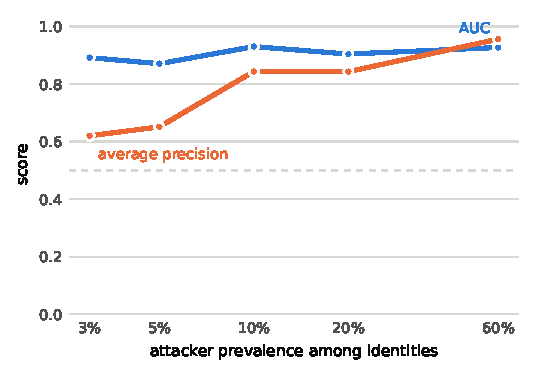
\includegraphics[width=\columnwidth]{fig_prevalence.pdf}
\caption{The two metrics respond differently to prevalence.
Ranking is nearly flat; average precision is not.
A result reported at native prevalence does not transfer.
GridSybil dense, three seeds per point.}
\label{fig:prevalence}
\end{figure}



%%SENSITIVITY_TABLE%%

%%SENSITIVITY_TEXT%%

\section{VeReMi 2018 as a Physical-Layer Substrate}

Signal-strength methods appear in 33 indexed records.
They need received power, which the Extension omits.
VeReMi 2018 does contain populated received power.
It contains no Sybil families, only position falsification.
Neither VeReMi release therefore carries both together.

One dataset outside the VeReMi family does carry both.
Guven and Tay\c{s}i built it for exactly this gap~\cite{guven2024}.
It pairs simulated RSSI with several Sybil attack variants.
We could not evaluate it here.
Its repository carries an owner takedown and authorship-dispute notice.
All data and code were restricted when we sought access.
We report that as a fact about availability, not about quality.

We fitted log-distance path loss over 86\,919 links.
Benign claims are honest, so their distances are trustworthy.
Table~\ref{tab:pathloss} reports the benign-only and all-link fits.

\begin{table}[t]
\caption{Path-loss behaviour and detector performance, VeReMi 2018.
Brackets are 95\% intervals for the estimator on that row.
Free space would give $-20$\,dB/decade and exponent 2.0.
Chance is AUC 0.5, and the attacker base rate is 0.055.}
\label{tab:pathloss}
\centering
\scriptsize
\begin{tabular}{@{}lrr@{}}
\toprule
Quantity & Benign fit & All links \\
\midrule
Correlation, $\log_{10} d$ & $-0.639$ & $-0.633$ \\
Slope (dB/decade) & $-9.41$ & $-9.29$ \\
Path-loss exponent & 0.941 & 0.929 \\
Scatter, median (dB) & 3.56 & 3.57 \\
\midrule
AUC across folds & 0.524\,[.502,.547] & 0.530\,[.507,.553] \\
AUC out of fold & 0.493\,[.485,.501] & 0.499\,[.491,.507] \\
Average precision & 0.054 & 0.054 \\
\bottomrule
\end{tabular}
\end{table}

Nine decibels per decade is very shallow.
Median per-link scatter is another 3.6 decibels.
A tenfold position lie barely clears that noise.

We then implemented position verification properly.
Receivers were placed from their own position reports.
Residuals were summarised per link and classified.
Senders were partitioned into five folds, disjoint by construction.
Every link is therefore scored once, by an unseen model.

Two estimators are reported, each with its own interval.
Averaging AUC across the five folds gives 0.530.
Its interval across folds runs 0.507 to 0.553.
Pooling the out-of-fold scores instead gives one global ranking.
That ranking reaches 0.499, with interval 0.491 to 0.507.
DeLong and bootstrap intervals agree to three decimals.
Average precision is 0.054 against a 5.5\% base rate.

The gap between the two estimators is itself informative.
Fold-local ranking is weak; global ranking is indistinguishable from chance.
A deployed detector needs one threshold, not five.
Raw signal statistics without geometry reach 0.597.
That figure averages five sender-disjoint random splits.
It is a fold-average, so it compares with 0.530, not 0.499.

Refitting on benign links alone changed almost nothing.
The exponent moved from 0.929 to 0.941.
Fold-mean AUC moved from 0.530 to 0.524.
The conclusion is therefore not an artefact of that choice.

The attack tested is constant position falsification.
It is the most blatant lie available, and goes undetected here.
We therefore make a narrow claim about this substrate.
VeReMi 2018 cannot meaningfully validate signal-strength position verification.
Whether the method works on calibrated data is untested here.

\section{Do the Shortcuts Generalise?}
\label{sec:generalise}

Every result so far comes from one dataset family.
The obvious objection is that these are quirks of one artefact.
VeReMi NextGen is the right test of that.

It uses InTAS rather than LuST, a later generator, another attack.
It was built to address limitations of the earlier releases.
We ran the same measurements on its four scenarios.

\begin{table}[t]
\caption{The same measurements on VeReMi NextGen, four scenarios.
Alias is what a receiver sees; sender identifier is ground truth.}
\label{tab:nextgen}
\centering
\footnotesize
\begin{tabular}{@{}lrr@{}}
\toprule
Measurement & Extension & NextGen \\
\midrule
Alias encodes the sender & 86.5--100\% & 0.0\% \\
Linkage AUC from the alias & 0.999--1.000 & 0.494--0.506 \\
Benign identities that rotate & 0 & 0 \\
Message-count AUC, untrained & 0.993--0.996 & 0.972--0.996 \\
Median copies per transmission & 4--7 & 2--49 \\
AUC from the sender identifier & --- & 1.000 \\
\bottomrule
\end{tabular}
\end{table}

Table~\ref{tab:nextgen} separates what was fixed from what was not.

The identity leak is genuinely repaired.
The receiver-visible alias no longer encodes the sender.
Linkage from it sits at chance in all four scenarios.
The artefact we weight most heavily is gone.

Three things survive the redesign.
Benign identities still never rotate, so privacy stays unstudiable.
Receiver duplication persists, at a median of 2 to 49 copies.
Message count alone still reaches AUC 0.972 to 0.996.

%%NEXTGEN_IDS%%

This field is ground truth, so no receiver can use it.
It matters because published pipelines do key on that field.
That is stage S0 of our own cascade, reconstructed from practice.
Any pipeline touching it inherits a perfect shortcut.

One caveat limits what we can compare.
In NextGen a ghost carries its own sender identifier.
That field therefore names an identity, not a vehicle.
Vehicle-level prevalence is not recoverable from it.
We report identity-level figures only, and say so.

\section{Discussion}

\subsection{What should change}

We propose the cascade itself as a pre-publication check.
Any detector evaluated on these archives can be run through it.
A result that survives S0 to S6 has earned its number.
A result that collapses at S2 was reading the partition.
The released script takes an archive and a model flag.
It reports the ladder for whatever detector is supplied.
A logistic regression run through it behaves the same way.
That removal is followed by 0.096 there and 0.064 here.
The ladder is a property of the data, not of one model.

We also propose seven reporting rules.
State the attacker fraction and beacon rate always.
Name the attack family and the density used.
Report an ablation separating timing from geometry.
Compare against a single-scalar baseline first.
Match evidence per identity when comparing policies.
Use identity-free tokens and disjoint splits by vehicle.
Publish the prevalence sweep, not one operating point.

\subsection{What our own errors taught us}

Nine defects were found and corrected during this work.
Duplicate observations inflated every timing feature initially.
Vehicle identifiers repeat across independent simulation runs.
One comparison pitted a pooled view against a single observer.
A sampler emptied the positive class at large scale.
A fixed output filename silently overwrote earlier results.
A leakage feature was hashed before being offered as leakage.
A path-loss model was fitted on the links it should exclude.
A point estimate was printed beside an interval for another estimator.
A reported table was published with no script behind it.

One diagnostic recurred each time.
Results were too strong for the available signal.
In the linkage experiment no pair feature passed AUC 0.65.
A forest on those same features still reported 1.000.
That gap indicated leakage, and leakage was present.

\section{Limitations}

Our audit covers the Sybil archives specifically.
Other attack families may behave differently.
Our controls use one detector family per experiment.
Stronger detectors could change absolute values.

Three threats deserve naming rather than listing.

Simulation realism bounds everything we report.
These archives model propagation and mobility, not radios.
A shortcut present in simulation need not survive on hardware.
Equally, hardware may add shortcuts a simulator never shows.

Jitter is applied afterwards to logged transmission times.
It therefore ignores medium access and collisions.
A real jittering attacker would interact with the channel.
Our jitter is an upper bound on how cheap the escape is.
We report it as one distribution, uniform, not as a model.

Observations are not independent within a vehicle.
Consecutive beacons from one sender are strongly correlated.
Our splits are vehicle-disjoint, which handles the worst of that.
Temporal dependence remains within folds.
Uncertainty estimates are therefore optimistic.

Two further limits are structural.
Emulated infrastructure uses claimed positions for reception.
That choice favours the infrastructure observer.
The prevalence floor is 3\% dense and 5\% sparse.
That limit is a property of the data, not our method.

External validity now rests on two datasets, not one.
Section~\ref{sec:generalise} tests the shortcuts on NextGen.
Both remain simulator output from one research lineage.

\section{Conclusion}

We measured what the VeReMi benchmarks contain.
Pseudonyms encode sender identity almost everywhere.
Honest vehicles never change pseudonyms in these archives.
Attacker prevalence is fixed at thirty percent throughout.
Ground-truth files omit most pseudonyms the attackers emitted.
One untrained scalar solves six of eight archives.
Timing alone reaches near-perfect linkage accuracy.
Geometry, the meaningful signal, performs far worse.

We then staged the protocol from published practice to deployment.
Removing ground-truth aggregation moved the score furthest.
The pseudonym feature added nothing once aggregation was fixed.
Ranking metrics survive a prevalence change; precision metrics do not.
Finally, VeReMi 2018 cannot validate the signal-strength family.
An accessible calibrated dataset is therefore a necessity.

Our code, controls and checklist accompany this paper.
We hope future results become comparable again.

\section*{Ethics}

This work analyses published artefacts and published papers.
It involves no human subjects and no personal data.
The archives are simulated, so no vehicle or driver is real.

We name specific papers in Table~\ref{tab:touch}.
We do so to locate protocol choices, not to allege misconduct.
Those choices were reasonable given what was documented.
Several are choices we made ourselves and later corrected.

We also describe a dataset withdrawn under an authorship dispute.
We report only its stated availability, which is a public fact.
We take no position on the dispute itself.
We did not obtain, mirror or redistribute that data.

\section*{Availability}

Scripts, controls and result tables are released with this paper.
They reproduce every number above from the raw archives.
The archive is deposited at \url{10.5281/zenodo.22397725}.
A container image rebuilds and re-verifies it in one command.
The full eight-archive census ships as a machine-readable table.
Every statistic we measured is a column, not only those printed here.

The route from raw data to results has four steps.
First, verify archive checksums against the Zenodo records.
Second, parse archives into cached views and ground truth.
Third, recover pseudonyms so the leakage arm is honest.
Fourth, run the numbered experiments in any order.

Every result file names the script that produced it.
A manifest records a hash per file and the library versions.
Independent metric implementations are included and self-tested.
